%%
%% AEGIS-Dengue long paper draft. Extends docs/short paper.tex with the
%% long-horizon benchmark of 24 September 2026 (docs/long_horizon_benchmark.md,
%% results/benchmark/). Every number below is taken from
%% results/benchmark/tables/*.csv or from the short paper's verified tables.
%%
%% TODO(team): Sections 6-10 use the Open-Meteo ERA5 reconstruction of the
%% climate inputs (district centroids). If the original Google Earth Engine
%% ERA5-Land extraction is recovered, rerun scripts 31-36 and update the
%% numbers marked in results/benchmark/tables before submission.
%%
% The bibliography is embedded so this single file compiles on its own (Prism,
% Overleaf or a local install): LaTeX writes references_long.bib on the first run.
\begin{filecontents*}[overwrite]{references_long.bib}
%% Bibliography for docs/long paper.tex.
%% The first eight entries are the short paper's references (reconstructed from its
%% printed reference list; replace them with the Overleaf references.bib entries if
%% those differ). Entries marked "VERIFY" had details not confirmed from the source
%% page during drafting — check author lists, volume and pages before submission.

@inproceedings{cho2014gru,
  author    = {Kyunghyun Cho and Bart van Merri{\"e}nboer and Caglar Gulcehre and Dzmitry Bahdanau and Fethi Bougares and Holger Schwenk and Yoshua Bengio},
  title     = {Learning Phrase Representations using {RNN} Encoder--Decoder for Statistical Machine Translation},
  booktitle = {Proceedings of the 2014 Conference on Empirical Methods in Natural Language Processing (EMNLP)},
  pages     = {1724--1734},
  year      = {2014},
  doi       = {10.3115/v1/D14-1179}
}

@article{funk2015chirps,
  author  = {Chris Funk and Pete Peterson and Martin Landsfeld and Diego Pedreros and James Verdin and others},
  title   = {The Climate Hazards Infrared Precipitation with Stations---A New Environmental Record for Monitoring Extremes},
  journal = {Scientific Data},
  volume  = {2},
  pages   = {150066},
  year    = {2015},
  doi     = {10.1038/sdata.2015.66}
}

@inproceedings{kingma2015adam,
  author    = {Diederik P. Kingma and Jimmy Ba},
  title     = {Adam: A Method for Stochastic Optimization},
  booktitle = {International Conference on Learning Representations (ICLR)},
  year      = {2015}
}

@inproceedings{kipf2017gcn,
  author    = {Thomas N. Kipf and Max Welling},
  title     = {Semi-Supervised Classification with Graph Convolutional Networks},
  booktitle = {International Conference on Learning Representations (ICLR)},
  year      = {2017}
}

@inproceedings{loshchilov2019decoupled,
  author    = {Ilya Loshchilov and Frank Hutter},
  title     = {Decoupled Weight Decay Regularization},
  booktitle = {International Conference on Learning Representations (ICLR)},
  year      = {2019}
}

@article{munoz2021era5land,
  author  = {Joaqu{\'i}n Mu{\~n}oz-Sabater and Emanuel Dutra and Anna Agust{\'i}-Panareda and Cl{\'e}ment Albergel and others},
  title   = {{ERA5-Land}: A State-of-the-Art Global Reanalysis Dataset for Land Applications},
  journal = {Earth System Science Data},
  year    = {2021},
  doi     = {10.5194/essd-13-4349-2021}
}

@manual{talagala2026denguedatahub,
  author = {Thiyanga S. Talagala},
  title  = {denguedatahub: A Tidy Format Datasets of Dengue by Country},
  note   = {R package version 4.1.0},
  year   = {2026},
  doi    = {10.32614/CRAN.package.denguedatahub}
}

@inproceedings{wu2019graph,
  author    = {Zonghan Wu and Shirui Pan and Guodong Long and Jing Jiang and Chengqi Zhang},
  title     = {Graph {WaveNet} for Deep Spatial-Temporal Graph Modeling},
  booktitle = {Proceedings of the 28th International Joint Conference on Artificial Intelligence (IJCAI)},
  pages     = {1907--1913},
  year      = {2019},
  doi       = {10.24963/ijcai.2019/264}
}

%% ---------------------------------------------------------------------------
%% New references for the long paper
%% ---------------------------------------------------------------------------

@inproceedings{weng2024graph,
  author    = {Jiaqi Weng and David Qiu and Ethan Cruz and Malik Magdon-Ismail and Thilanka Munasinghe and Jennifer C. Wei and Ashan Pathirana},
  title     = {Graph Representation Learning for Dengue Forecasting},
  booktitle = {2024 IEEE International Conference on Big Data (BigData)},
  pages     = {4448--4456},
  year      = {2024},
  doi       = {10.1109/BigData62323.2024.10825335}
}

@article{gulmohamed2026denguegnn,
  author  = {Rasitha Banu GulMohamed and Wafa Hetany and Hanan Abdullah Almaimani and Faiza Abdalla Saeed Khiery},
  title   = {{DengueGNN}: Graph-based deep learning for modeling disease spread dynamics and prediction},
  journal = {Scientific Reports},
  volume  = {16},
  pages   = {10584},
  year    = {2026},
  doi     = {10.1038/s41598-026-43073-y}
}

@article{liu2025explainable,
  author  = {Yichao Liu and Peter Fransson and Julian Heidecke and Prasad Liyanage and Jonas Wallin and Joacim Rockl{\"o}v},
  title   = {An explainable covariate compartmental model for predicting the spatio-temporal patterns of dengue in {Sri Lanka}},
  journal = {PLoS Computational Biology},
  volume  = {21},
  number  = {9},
  pages   = {e1013540},
  year    = {2025},
  doi     = {10.1371/journal.pcbi.1013540},
  note    = {VERIFY first names}
}

@article{johansson2019open,
  author  = {Michael A. Johansson and Karyn M. Apfeldorf and Scott Dobson and others},
  title   = {An open challenge to advance probabilistic forecasting for dengue epidemics},
  journal = {Proceedings of the National Academy of Sciences},
  volume  = {116},
  number  = {48},
  pages   = {24268--24274},
  year    = {2019},
  doi     = {10.1073/pnas.1909865116}
}

@article{bracher2021evaluating,
  author  = {Johannes Bracher and Evan L. Ray and Tilmann Gneiting and Nicholas G. Reich},
  title   = {Evaluating epidemic forecasts in an interval format},
  journal = {PLoS Computational Biology},
  volume  = {17},
  number  = {2},
  pages   = {e1008618},
  year    = {2021},
  doi     = {10.1371/journal.pcbi.1008618}
}

@article{mosqlimate2026sprint,
  author  = {{Infodengue-Mosqlimate Dengue Forecasting Sprint Consortium}},
  title   = {Leveraging probabilistic forecasts for dengue preparedness and control: The 2024 Dengue Forecasting Sprint in {Brazil}},
  journal = {Proceedings of the National Academy of Sciences},
  year    = {2026},
  doi     = {10.1073/pnas.2508989123},
  note    = {VERIFY author list and year}
}

@article{colongonzalez2021probabilistic,
  author  = {Felipe J. Col{\'o}n-Gonz{\'a}lez and Leonardo Soares Bastos and Barbara Hofmann and others},
  title   = {Probabilistic seasonal dengue forecasting in {Vietnam}: A modelling study using superensembles},
  journal = {PLoS Medicine},
  volume  = {18},
  number  = {3},
  pages   = {e1003542},
  year    = {2021},
  doi     = {10.1371/journal.pmed.1003542}
}

@article{ensemble2025global,
  author  = {{VERIFY}},
  title   = {Ensemble approaches for short-term dengue fever forecasts: A global evaluation study},
  year    = {2025},
  note    = {PMC12377650. VERIFY authors, journal and volume},
  url     = {https://pmc.ncbi.nlm.nih.gov/articles/PMC12377650/}
}

@inproceedings{ke2017lightgbm,
  author    = {Guolin Ke and Qi Meng and Thomas Finley and Taifeng Wang and Wei Chen and Weidong Ma and Qiwei Ye and Tie-Yan Liu},
  title     = {{LightGBM}: A Highly Efficient Gradient Boosting Decision Tree},
  booktitle = {Advances in Neural Information Processing Systems (NeurIPS)},
  year      = {2017}
}

@article{ansari2024chronos,
  author  = {Abdul Fatir Ansari and Lorenzo Stella and Caner Turkmen and others},
  title   = {Chronos: Learning the Language of Time Series},
  journal = {Transactions on Machine Learning Research},
  year    = {2024}
}

@misc{ansari2025chronos2,
  author = {Abdul Fatir Ansari and others},
  title  = {Chronos-2: From Univariate to Universal Forecasting},
  year   = {2025},
  note   = {Amazon Science technical report. VERIFY arXiv identifier},
  url    = {https://github.com/amazon-science/chronos-forecasting}
}

@inproceedings{hu2022lora,
  author    = {Edward J. Hu and Yelong Shen and Phillip Wallis and Zeyuan Allen-Zhu and Yuanzhi Li and Shean Wang and Lu Wang and Weizhu Chen},
  title     = {{LoRA}: Low-Rank Adaptation of Large Language Models},
  booktitle = {International Conference on Learning Representations (ICLR)},
  year      = {2022}
}

@book{vovk2005algorithmic,
  author    = {Vladimir Vovk and Alexander Gammerman and Glenn Shafer},
  title     = {Algorithmic Learning in a Random World},
  publisher = {Springer},
  year      = {2005}
}
\end{filecontents*}
\documentclass[sigconf,nonacm]{acmart}

\AtBeginDocument{%
  \providecommand\BibTeX{{%
    Bib\TeX}}}

\usepackage{hyperref}
\usepackage{graphicx}
\usepackage{booktabs}
\usepackage{tikz}
\usetikzlibrary{positioning,arrows.meta}

% Figures: copy results/benchmark/figures/*.pdf and figures/fig_h1_landscape.pdf
% into figures/ (or images/ on Overleaf).
\graphicspath{{images/}{../figures/}{figures/}{./}}

\setlength{\textfloatsep}{6pt plus 2pt minus 2pt}
\setlength{\intextsep}{6pt plus 2pt minus 2pt}
\settopmatter{printacmref=false}
\renewcommand\footnotetextcopyrightpermission[1]{}
\pagestyle{plain}
% Lets TeX stretch interword space slightly instead of overrunning the column
% on lines with long hyphenated terms.
\setlength{\emergencystretch}{1.5em}

\begin{document}

\title{How Far Ahead Can We Warn? A Leakage-Controlled Benchmark of Graph, Recurrent, Tabular and Foundation Models for District-Level Dengue Forecasting in Sri Lanka}

% acmart wants one \author per person, each with its own affiliation.
\newcommand{\uom}{\affiliation{%
  \institution{Department of Computer Science and Engineering}
  \institution{University of Moratuwa}
  \country{Sri Lanka}}}
\author{Kulathunge K. A. N. H.}\uom\email{nadilk.23@cse.mrt.ac.lk}
\author{Angeesa R. P. T.}\uom\email{thilokyaa.23@cse.mrt.ac.lk}
\author{Gunaweera N.}\uom\email{nethsithg.23@cse.mrt.ac.lk}
\author{Mallawarachchi H. S.}\uom\email{hesandim.23@cse.mrt.ac.lk}
\author{Wijesekara M. S. T.}\uom\email{senilkam.23@cse.mrt.ac.lk}

\renewcommand{\shortauthors}{Kulathunge et al.}

\begin{abstract}
Dengue forecasting studies for Sri Lanka report graph neural networks outperforming ARIMA, random forests and LSTMs, but rarely compare against persistence, the forecast that simply repeats the latest count. We build a leakage-controlled benchmark over 25 districts and nineteen years of weekly surveillance, with ten walk-forward folds, horizons of 1--12 weeks, and 24 forecasters scored on identical district-weeks: graph-convolutional and recurrent networks, gradient-boosted trees, linear autoregression, and the pretrained time-series foundation models Chronos-Bolt and Chronos-2, zero-shot and fine-tuned. At one week ahead persistence is hard to beat; a GRU trained with a level-weighted quantile loss is the first configuration to do so on the headline mean (15.70 vs 16.42 MAE, $p=0.045$), though not after correction for multiple comparisons. From three weeks ahead almost every learned model beats persistence significantly, with skill rising to 19--25\% at 12 weeks. A zero-shot Chronos-2 matches our purpose-built GRU without seeing any dengue data. Capacity-matched ablations in three model families show that climate reduces error from about two to four weeks ahead onward, and that the effect persists to 12 weeks. Spatial graphs, fixed or learned, never help. Native quantile forecasts improve the weighted interval score by 27--33\% over persistence with near-nominal coverage. Finally, models discriminate outbreak weeks well (AUC 0.91 at one week) but are close to chance at predicting outbreak \emph{onsets} (AUC 0.53--0.63), a gap that standard early-warning evaluations hide.
\end{abstract}

\maketitle

%% ---------------------------------------------------------------------------
\section{Introduction}

Weekly district-level dengue surveillance can support earlier public-health action when forecasts give useful lead time before a surge. Vector-control resources of the National Dengue Control Unit (NDCU) and Public Health Inspectors (PHIs), hospital staffing and ward capacity all need lead times of several weeks, and Sri Lanka's 2017 epidemic, the largest on record, showed the cost of reacting late.

Two features of the forecasting problem shape how it should be evaluated. First, at one week ahead the most recent count is already a very strong predictor, so any claim of skill must be measured against \emph{persistence} rather than against other learned models. Second, climate acts on dengue through the mosquito life cycle with a delay of several weeks; the rainfall-to-dengue delay we measure is 5--10 weeks, in line with the 7--9 weeks reported for Sri Lanka by Liu et al.~\cite{liu2025explainable}. A benchmark that stops at one or four weeks cannot see where climate matters.

Recent Sri Lankan work reports spatio-temporal graph neural networks outperforming ARIMA, random forests and LSTMs~\cite{weng2024graph,gulmohamed2026denguegnn}, but without a persistence baseline, walk-forward evaluation over multiple epidemic regimes, or probabilistic scoring. Operational dengue forecasting elsewhere has moved to probabilistic forecasts scored by proper scoring rules~\cite{johansson2019open,bracher2021evaluating,mosqlimate2026sprint} and to ensembles~\cite{colongonzalez2021probabilistic}. Meanwhile, pretrained time-series foundation models~\cite{ansari2024chronos,ansari2025chronos2} offer strong zero-shot forecasts but have not been tested on dengue in Sri Lanka.

\textbf{Contributions.}
\begin{enumerate}
\item A leakage-controlled benchmark of 24 forecasters for 25 districts at horizons of 1--12 weeks, scored on identical district-weeks, with a calibration fold so that intervals, ensemble weights and alarm cutoffs are never fitted on the scored year.
\item Evidence that persistence dominates at one week (with one promising exception) and that skill from three to twelve weeks is robust against persistence and strong machine-learning baselines.
\item The first comparison, to our knowledge, of pretrained time-series foundation models with purpose-built models for dengue in Sri Lanka: zero-shot Chronos-2 matches our best GRU.
\item Capacity-matched climate ablations in three model families showing climate helps from two to four weeks ahead onward and keeps helping to twelve weeks.
\item Negative results on spatial structure: neither fixed nor learned graphs help at any horizon.
\item Calibrated probabilistic forecasts, and an early-warning evaluation that separates outbreak weeks from outbreak onsets and shows onsets remain close to unpredictable.
\end{enumerate}

%% ---------------------------------------------------------------------------
\section{Related Work}

\textbf{Dengue forecasting in Sri Lanka.} Weng et al.~\cite{weng2024graph} compare five spatio-temporal GNNs with ARIMAX, random forests, XGBoost and LSTMs for the 25 districts over 2013--2022, forecasting three weeks from a three-week window, and find the GNNs best; their evaluation uses a 70/30 split within rolling segments and no persistence baseline. GulMohamed et al.~\cite{gulmohamed2026denguegnn} propose a dynamic graph with mobility priors and attention-augmented LSTMs. Liu et al.~\cite{liu2025explainable} combine an SEIR model with an LSTM that estimates the force of infection for 16 aggregated districts, identifying 7--9 week lags for precipitation and temperature.

\textbf{Evaluation of epidemic forecasts.} The dengue forecasting challenge of Johansson et al.~\cite{johansson2019open} and the 2024 Brazilian Dengue Forecasting Sprint~\cite{mosqlimate2026sprint} score probabilistic forecasts with proper scoring rules; the weighted interval score (WIS)~\cite{bracher2021evaluating} is now standard. Colón-González et al.~\cite{colongonzalez2021probabilistic} show that superensembles beat a baseline in Vietnam at one to three months but not beyond. A multi-country study finds weighted ensembles most often among the best models~\cite{ensemble2025global}.

\textbf{Models.} Graph convolution~\cite{kipf2017gcn} and GRUs~\cite{cho2014gru} are the standard spatio-temporal building blocks; Graph WaveNet~\cite{wu2019graph} learns the adjacency end-to-end. Gradient-boosted trees~\cite{ke2017lightgbm} are strong tabular forecasters. Chronos~\cite{ansari2024chronos} tokenises series and pretrains a language-model architecture on large corpora; Chronos-2~\cite{ansari2025chronos2} adds covariates and multivariate group attention. We fine-tune it with LoRA~\cite{hu2022lora}.

%% ---------------------------------------------------------------------------
\section{Data}
\label{sec:data}

\textbf{Dengue cases.} Weekly confirmed counts come from the denguedatahub repository~\cite{talagala2026denguedatahub}. The 26 reporting areas are consolidated into 25 districts by merging Kalmunai into Ampara. The panel spans 1,012 reporting periods from December 2006 to May 2026. Unobserved district-weeks (one Puttalam record) are masked, never imputed.

\textbf{Climate.} Daily rainfall, 2\,m temperature (mean, minimum, maximum), dew point, relative humidity and wind speed are aggregated to the reporting calendar. The experiments of Section~\ref{sec:h1} use ERA5-Land~\cite{munoz2021era5land} polygon means extracted through Google Earth Engine, validated against CHIRPS~\cite{funk2015chirps}. The benchmark of Sections~\ref{sec:benchmark}--\ref{sec:ews} uses the same reanalysis family served by Open-Meteo (ERA5-Land for temperature, dew point and humidity; ERA5 for rainfall and wind) at each district's centroid. Case data, folds and persistence are identical in both: persistence reproduces 16.42, 20.16, 24.58 and 28.47 MAE at $h=1$--4 exactly, and the GRU at $h=4$ scores 25.30 with the reconstruction against 25.40 with the original extraction.

\textbf{Features.} Variant v0 holds log cases, climate, season (day-of-year sine and cosine), observation flags and centroid coordinates. v1 adds trailing 4/8/12-week means of rainfall, temperature and humidity. v2 adds two outbreak-history features: each district's weekly rank among the 25 districts and its log trailing 52-week case total.

%% ---------------------------------------------------------------------------
\section{Methods}
\label{sec:methods}

\subsection{Task and target}
For a forecast origin $t$ and horizon $h\in\{1,2,3,4,6,8,10,12\}$ each model predicts $y_{t+h}$ for every district from data up to $t$. Neural and tabular models predict the anchored log residual
\[
\Delta_{t,h}=\log(1+y_{t+h})-\log(1+y_t),
\]
so a zero prediction reproduces persistence. One model is trained per horizon.

\subsection{GCN--GRU and variants}
Each input week passes through graph convolution over the 25 districts, a shared GRU encodes the 12-week window per district, and a linear head predicts the residual (Figure~\ref{fig:pipeline}). Replacing the adjacency with the identity turns the graph convolution into a per-district layer; this identity backbone is the GRU control. We vary the adjacency (identity, queen contiguity, Gaussian distance, learned Graph WaveNet adjacency~\cite{wu2019graph}), the features (v1, v2) and the loss: masked MSE, a pinball loss over seven quantile levels from 0.025 to 0.975 (the median and the 50\%, 80\% and 95\% central intervals), whose median is the point forecast, and level weighting, which weights each cell by $\log(1+y_t)$ normalised to mean one per batch.

\begin{figure}[t]
\centering
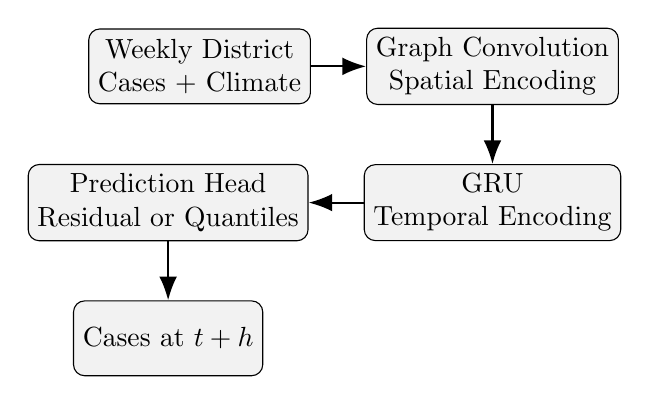
\begin{tikzpicture}[
    node distance=0.85cm,
    box/.style={draw, rounded corners, minimum width=2.0cm, minimum height=0.95cm, align=center, fill=gray!10},
    arrow/.style={-{Latex[length=3mm]}, thick}]
\node[box] (input) {Weekly District\\Cases + Climate};
\node[box, right=0.7cm of input] (gcn) {Graph Convolution\\Spatial Encoding};
\node[box, below=0.75cm of gcn] (gru) {GRU\\Temporal Encoding};
\node[box, left=0.7cm of gru] (head) {Prediction Head\\Residual or Quantiles};
\node[box, below=0.75cm of head] (final) {Cases at $t+h$};
\draw[arrow] (input) -- (gcn);
\draw[arrow] (gcn) -- (gru);
\draw[arrow] (gru) -- (head);
\draw[arrow] (head) -- (final);
\end{tikzpicture}
\caption{GCN--GRU forecaster. The adjacency is varied between identity, geographic contiguity, Gaussian distance and a learned graph; the head outputs either one residual or seven quantiles.}
\label{fig:pipeline}
\Description{Flow diagram: weekly district cases and climate pass through graph convolution, then a GRU, then a prediction head that outputs a residual or seven quantiles, giving cases at week t plus h.}
\end{figure}

\subsection{Baselines}
\textbf{Naive.} Persistence ($y_t$); seasonal naive ($y_{t+h-52}$); climatology (geometric mean of the same week in the previous five years); seasonal persistence (persistence shifted by the typical seasonal change from origin to target week).

\textbf{Tabular.} A global LightGBM~\cite{ke2017lightgbm} and a ridge autoregression (ARX) predict the same residual from v2 features, log-case lags 1--12, rolling means and maxima, 4-week rainfall, humidity and temperature means lagged 4 and 8 weeks and 12-week rainfall lagged 12 weeks, neighbour and national case levels, the target week's season and a district identifier.

\textbf{Foundation models.} Chronos-Bolt-small and Chronos-2~\cite{ansari2024chronos,ansari2025chronos2} forecast $\log(1+y)$ from each district's full history, zero-shot. Chronos-2 is also run with past four-week climate means as covariates and the target week's season as a known future covariate, and \emph{jointly}, with the 25 districts as one multivariate series. Fine-tuned variants apply LoRA~\cite{hu2022lora} per fold on data up to the training cut-off only; the number of steps (1,000 of $\{100,300,1000\}$) was chosen once on the 2015 validation year of a calibration fold.

\textbf{Ensembles.} An equal-weight ensemble of GRU~v2, LightGBM and Chronos-2 fixed in advance; a stacked ensemble with non-negative least-squares weights; and a top-3 ensemble that averages the three forecasters with the lowest MAE in the previous test year. All combine in log space.

\subsection{Evaluation protocol}
\textbf{Folds.} Walk-forward folds with expanding training history test on each calendar year 2016--2025; the preceding year is the validation year used for early stopping. Fold 0 (2016) is used only for calibration. Headline figures average the seven non-COVID test years (2017, 2018, 2019, 2022, 2023, 2024, 2025); 2017 is the epidemic year. Per-fold imputation and scaling are fitted on data before the test year.

\textbf{Common cells.} Every method is scored on the identical 208,800 (fold, split, horizon, week, district) cells. Anything calibrated for test year $f$ (conformal intervals, stacking weights, top-3 membership, alarm cutoffs) uses the out-of-sample forecasts for year $f-1$.

\textbf{Metrics.} MAE and peak MAE on raw counts, where peak cells are those at or above the district's 90th percentile of pre-test history; WIS~\cite{bracher2021evaluating} and 95\% interval coverage; ROC-AUC for outbreak weeks (peak cells) against all other weeks, and for \emph{onsets}, the first outbreak week after at least four quiet weeks, against quiet weeks. Point models receive intervals by split-conformal calibration~\cite{vovk2005algorithmic} of log residuals on the previous year.

\textbf{Statistics.} Trained models use three seeds. Differences are paired over the seven headline years with a $t$-test and a Wilcoxon signed-rank test, and we report years won. With seven years the smallest attainable two-sided Wilcoxon $p$ is 0.016.

%% ---------------------------------------------------------------------------
\section{One Week Ahead}
\label{sec:h1}

This section summarises the one-week experiments on the original climate extraction, then the new one-week result from the benchmark.

\begin{table}[t]
\centering
\caption{One-week-ahead results over the seven headline folds (original climate extraction).}
\label{tab:h1baseline}
\begin{tabular}{lccccc}
\toprule
\textbf{Model} & \textbf{Feat.} & \textbf{MAE} & \textbf{RMSE} & \textbf{Peak} & \textbf{2017} \\
\midrule
Persistence & -- & \textbf{16.42} & \textbf{33.61} & \textbf{26.61} & \textbf{36.08} \\
GRU only & v1 & 16.68 & 35.25 & 28.06 & 42.97 \\
GRU only & v0 & 16.86 & 35.94 & 28.43 & 43.53 \\
GCN+GRU & v0 & 18.60 & 39.68 & 29.81 & 51.87 \\
GCN+GRU & v1 & 18.98 & 40.36 & 30.36 & 54.81 \\
\bottomrule
\end{tabular}
\end{table}

No trained model beat persistence on the headline mean (Table~\ref{tab:h1baseline}). The GRU-only control beat the geographic GCN--GRU on every fold, so contiguity is not neutral: it costs accuracy. Figure~\ref{fig:h1} places every one-week configuration against persistence. Each intervention produced the same pattern: a gain concentrated in the 2017 epidemic fold and no change elsewhere.
\begin{itemize}
\item \textbf{Learnable climate lags.} A per-district 26-week delay kernel recovered planted synthetic delays but not the measured 5--10 week delays when trained end-to-end (learned vs measured $r=-0.16$; 20.67 MAE vs 18.36 for fixed windows). Removing all climate at $h=1$ changed MAE on recent normal folds by only $+0.01$.
\item \textbf{Losses.} Level weighting cut GCN--GRU MAE from 18.98 to 16.59, entirely from the 2017 fold.
\item \textbf{Hyperparameters and optimisers.} A 50-trial search over nine axes gained 0.75 MAE, under two seed standard deviations; AdamW and plateau scheduling were within noise. In 23 of 27 scheduled runs the learning rate dropped only after early stopping had already fixed the best epoch.
\item \textbf{Graphs.} No graph beat the identity control (adaptive 16.61, identity 16.68, contiguity 18.98, Gaussian 19.25). A per-district gate between graph and no graph learned almost nothing.
\end{itemize}

\begin{figure}[t]
\centering
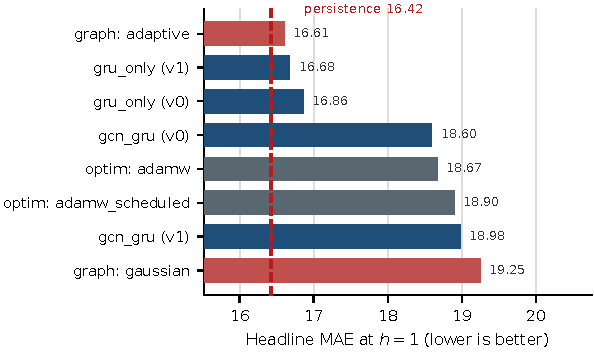
\includegraphics[width=\columnwidth]{fig_h1_landscape}
\caption{Every one-week configuration from the earlier study against the persistence baseline (dashed).}
\label{fig:h1}
\Description{Horizontal bar chart of one-week MAE for every configuration from the earlier study; all bars sit at or to the right of the dashed persistence line at 16.42.}
\end{figure}

\textbf{A first one-week win.} In the benchmark, every learned model already beats persistence on all six non-epidemic headline years at $h=1$, by roughly one case per district-week; the headline mean is decided by 2017. Combining the quantile head with level weighting reduces the 2017 loss from $+6.87$ MAE (GRU~v2) to $+0.78$, and gives 15.70 MAE against 16.42 for persistence ($+4.4\%$ skill, paired $t$-test $p=0.045$, six of seven years won, Wilcoxon $p=0.11$). Zero-shot Chronos-2 joint also scores below persistence (15.95) but not significantly. Because this configuration is one of roughly 17 compared, the result does not survive a multiple-comparison correction and should be treated as promising rather than established.

%% ---------------------------------------------------------------------------
\section{Multi-Horizon Benchmark}
\label{sec:benchmark}

Table~\ref{tab:main} gives headline MAE for the main forecasters at each horizon; Figure~\ref{fig:skill} shows skill relative to same-horizon persistence, which degrades from 16.42 MAE at one week to 46.47 at twelve.

\begin{table*}[t]
\centering
\caption{Headline MAE (cases per district-week, mean over the seven headline test years) by forecast horizon $h$ in weeks. Bold marks the lowest value per column. Three seeds per trained model.}
\label{tab:main}
\begin{tabular}{llccccccc}
\toprule
\textbf{Family} & \textbf{Method} & $h=1$ & $h=2$ & $h=3$ & $h=4$ & $h=6$ & $h=8$ & $h=12$ \\
\midrule
Naive & Persistence & 16.42 & 20.16 & 24.58 & 28.47 & 35.01 & 40.07 & 46.47 \\
 & Seasonal persistence & 23.19 & 26.36 & 30.16 & 32.90 & 37.20 & 42.66 & 48.16 \\
Tabular & Ridge ARX & 17.96 & 21.39 & 24.24 & 26.70 & 30.96 & 34.22 & 38.23 \\
 & LightGBM & 16.99 & 21.05 & 24.30 & 27.16 & 32.34 & 36.29 & 40.59 \\
GRU & GRU v1 (short paper) & 16.80 & 20.41 & 23.02 & 25.95 & 30.19 & 33.99 & 37.77 \\
 & GRU v2 & 16.64 & 19.51 & 22.33 & 25.30 & 30.85 & 34.33 & 38.10 \\
 & GRU v2, quantile + level-weighted & \textbf{15.70} & \textbf{19.00} & 22.38 & \textbf{24.58} & 29.94 & 33.10 & 37.94 \\
 & GCN v2 (contiguity graph) & 17.84 & 23.30 & 25.46 & 27.59 & 31.86 & 34.58 & 38.78 \\
Foundation & Chronos-Bolt, zero-shot & 16.60 & 20.19 & 23.63 & 26.41 & 30.50 & 33.42 & 36.69 \\
 & Chronos-2, zero-shot & 16.03 & 19.34 & 22.86 & 25.89 & 30.46 & 33.98 & 37.64 \\
 & Chronos-2 joint, zero-shot & 15.95 & 19.07 & \textbf{22.29} & 25.11 & 29.39 & 32.74 & 36.30 \\
 & Chronos-2 + climate, zero-shot & 16.71 & 19.56 & 22.57 & 24.93 & 29.22 & 32.38 & 35.86 \\
 & Chronos-2, fine-tuned & 18.59 & 21.07 & 23.59 & 25.63 & 29.26 & 31.74 & \textbf{34.76} \\
 & Chronos-2 joint, fine-tuned & 17.32 & 19.80 & 22.38 & 25.07 & \textbf{28.82} & \textbf{31.70} & 35.17 \\
Ensemble & Equal weights (pre-specified) & 16.05 & 19.27 & 22.30 & 25.01 & 29.79 & 33.19 & 36.82 \\
 & Top-3 by previous year & 15.90 & 20.82 & 23.00 & 25.22 & 28.91 & 32.39 & 36.48 \\
\bottomrule
\end{tabular}
\end{table*}

\begin{figure*}[t]
\centering
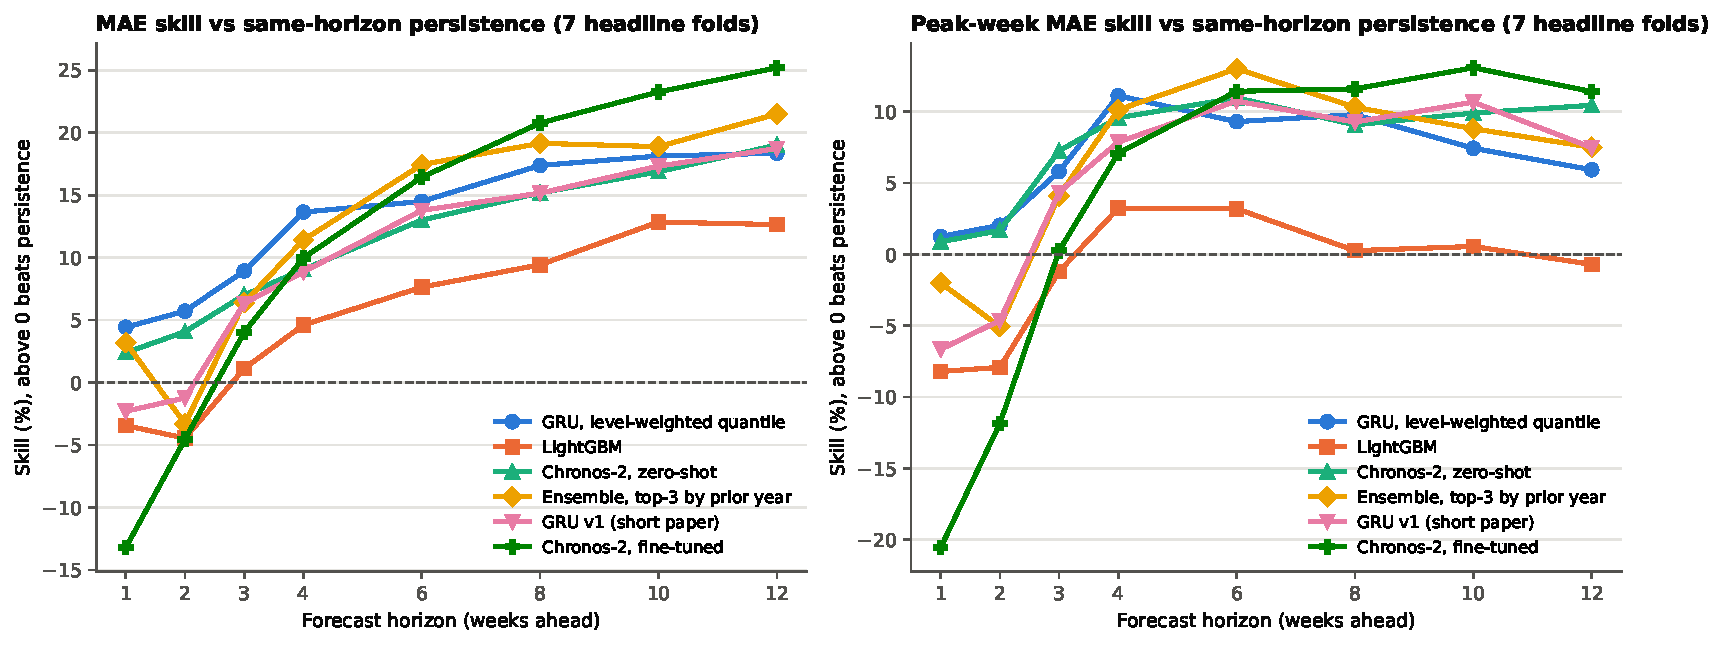
\includegraphics[width=\textwidth]{fig_lh_skill}
\caption{Skill relative to same-horizon persistence for MAE (left) and peak-week MAE (right), mean over the seven headline test years. Above zero beats persistence.}
\label{fig:skill}
\Description{Two line charts of skill versus forecast horizon from 1 to 12 weeks for six forecasters. Most lines start near or below zero at one week and rise to between 12 and 25 percent at 12 weeks.}
\end{figure*}

\textbf{Skill grows with horizon.} From $h=3$ onward nearly every learned model beats persistence, and the margin grows: at $h=4$ the quantile level-weighted GRU has 13.7\% MAE skill and the equal-weight ensemble 12.2\% ($p=0.003$); at $h=12$ the fine-tuned Chronos-2 reaches 25.2\%. From $h=4$ the Chronos arms and both zero-shot and fine-tuned variants win all seven years (Wilcoxon $p=0.016$). Peak-week skill follows the same shape but saturates near 10--13\% (Figure~\ref{fig:skill}, right).

\textbf{Foundation models.} Chronos-2 never saw dengue or Sri Lanka, yet forecasting the 25 districts jointly it is within about 0.6 MAE of the best GRU at every horizon and beats persistence significantly from $h=2$ ($p=0.018$). Joint forecasting improves on univariate Chronos-2 at every horizon, by 0.1--1.5 MAE. Fine-tuning moves skill toward long horizons: it makes Chronos-2 the most accurate model at 6--12 weeks but costs 2.6 MAE at one week, almost all of it in 2017, where the fine-tuned model, trained only on the quieter years before the epidemic, under-predicts the surge.

\textbf{Tabular baselines.} LightGBM never beats persistence at one or two weeks and trails the GRU by 2--3 MAE from four weeks. The linear ARX is weak at short horizons but competitive at long ones. The comparison matters because the tree-based rows are the baselines against which earlier Sri Lankan GNNs were reported~\cite{weng2024graph}.

\textbf{Ensembles.} The pre-specified equal-weight ensemble is among the best at 2--4 weeks. Learned combination does not help: stacked weights are worse than equal weights at every horizon, and the top-3 ensemble's membership changes from year to year, so selection on the previous year transfers poorly, an instance of the forecast-combination puzzle.

%% ---------------------------------------------------------------------------
\section{What Climate Contributes}
\label{sec:climate}

\textbf{Design.} Removing climate channels changes the input width and parameter count as well as the information, so a removal penalty need not concern weather. We therefore use a shuffle control for the GRU: every climate-derived channel is permuted in time across whole windows, independently per district and channel, within each data split. Width, parameters, scaler statistics and marginal distributions are unchanged; only the weather-to-time alignment is destroyed. For LightGBM, removal is the clean ablation because trees do not share a first layer. For Chronos-2 we add climate as covariates to the zero-shot model.

\begin{table}[t]
\centering
\caption{Error reduction attributable to climate (MAE, cases per district-week; positive means climate helps), paired over seven headline years.}
\label{tab:climate}
\begin{tabular}{lccc}
\toprule
$h$ & \textbf{GRU} (shuffle) & \textbf{LightGBM} (remove) & \textbf{Chronos-2} (add) \\
\midrule
1 & $+0.01$ & $+0.40$ & $-0.68$ \\
2 & $+1.03$ & $+0.64$ & $-0.22$ \\
3 & $+1.97$ & $+0.46$ & $+0.29$ \\
4 & $+1.91$ & $+0.63$ & $+0.96$ \\
6 & $+1.14$ & $+0.66$ & $+1.24$ \\
8 & $+1.50$ & $+0.47$ & $+1.60$ \\
10 & $+2.29$ & $+0.84$ & $+1.88$ \\
12 & $+2.46$ & $+0.52$ & $+1.78$ \\
\bottomrule
\end{tabular}
\end{table}

\begin{figure*}[t]
\centering
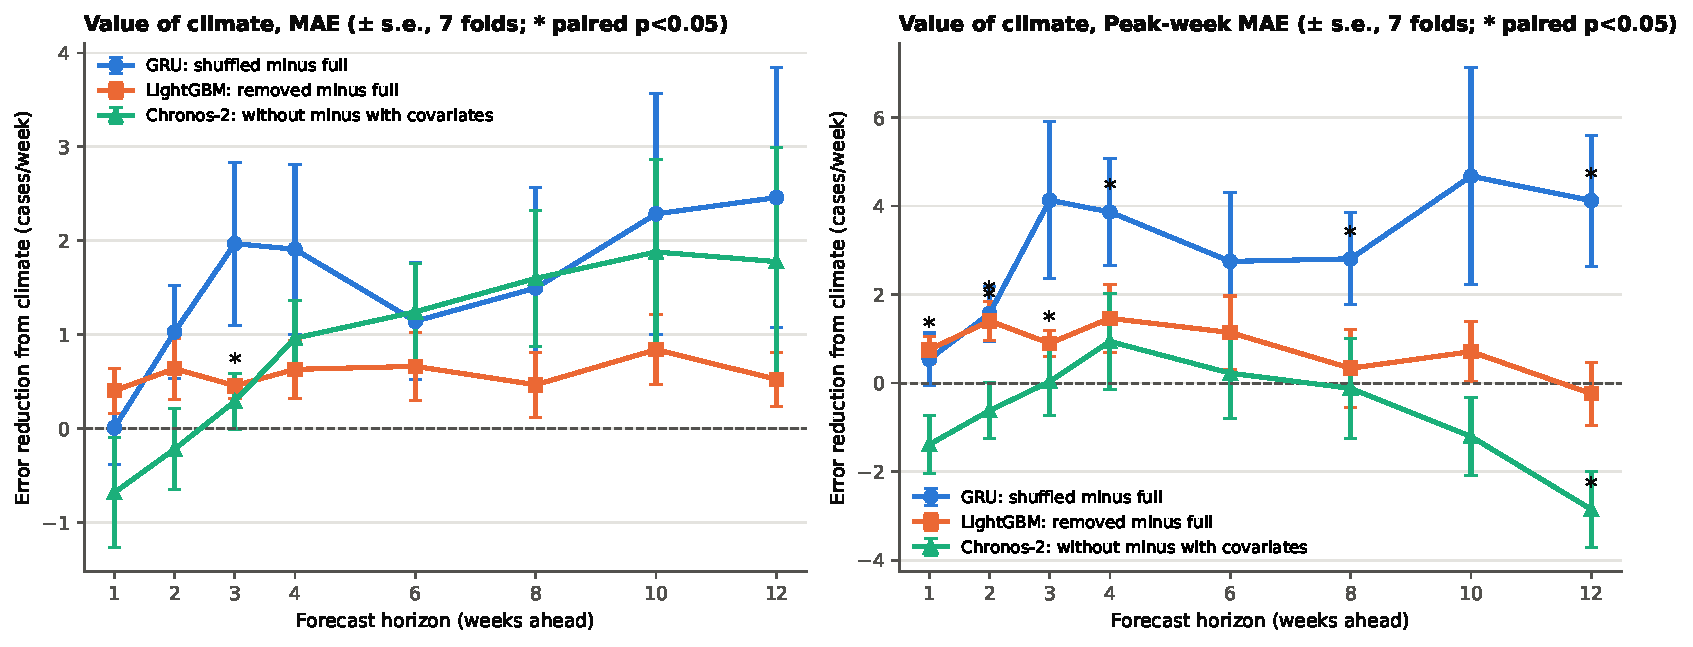
\includegraphics[width=\textwidth]{fig_lh_climate}
\caption{Error reduction attributable to climate in three model families, for MAE (left) and peak-week MAE (right), $\pm$ standard error over seven headline years; * marks paired $p<0.05$.}
\label{fig:climate}
\Description{Two line charts of error reduction attributable to climate versus horizon for a GRU, LightGBM and Chronos-2. All three are near zero or negative at one week and positive from about two to four weeks onward.}
\end{figure*}

\textbf{Results.} In all three families climate contributes from about two to four weeks ahead (Table~\ref{tab:climate}, Figure~\ref{fig:climate}). For the GRU, shuffling costs nothing at one week and 1.0--2.5 MAE from two weeks on, hurting in six of seven years at 2, 3 and 12 weeks; the peak-week cost is 1.6--4.7 MAE and significant at 2, 4, 8 and 12 weeks. For LightGBM, removal costs 0.4--0.8 MAE at every horizon (Wilcoxon $p\le0.031$ at $h=1$--3). Chronos-2 is hurt by climate covariates at one week but helped from four weeks on, in six of seven years ($p\approx0.05$). The GRU result at four weeks ($+1.91$) replicates the earlier ablation on the original climate extraction ($+1.55$, $p=0.016$), where the removal arm alone was weak and negative at $h=1$--3; without the shuffle control, the opposite conclusion would have been drawn.

\textbf{A refuted hypothesis.} We expected climate's value to peak near the 5--10 week biological delay and fade beyond it, since weather that affects the target week has not yet occurred at longer horizons. It does not fade by twelve weeks. A likely explanation is that past climate at the origin also encodes the phase and strength of the monsoon season, which remains informative about transmission months later. Individual per-horizon tests are mostly at $p=0.06$--0.2; the evidence is the consistency across horizons and across three unrelated model families.

%% ---------------------------------------------------------------------------
\section{Spatial Structure}
\label{sec:spatial}

\begin{table}[t]
\centering
\caption{MAE change from adding a graph to the GRU~v2 (positive means the graph hurts).}
\label{tab:graphs}
\begin{tabular}{lccccc}
\toprule
\textbf{Graph} & $h=1$ & $h=2$ & $h=4$ & $h=8$ & $h=12$ \\
\midrule
Contiguity & $+1.20$ & $+3.78$ & $+2.29$ & $+0.25$ & $+0.68$ \\
Learned (adaptive) & $+0.49$ & $+5.58$ & $+1.61$ & $+1.61$ & $+1.27$ \\
\bottomrule
\end{tabular}
\end{table}

Neither the contiguity graph nor an adjacency learned end-to-end helps at any horizon (Table~\ref{tab:graphs}); the learning rate of the learned graph was selected per fold and horizon on the validation year. The contiguity penalty shrinks with horizon, from 3.8 MAE at two weeks to 0.3--0.7 at eight to twelve, but never becomes a gain. Cross-district information is nonetheless useful in another form: Chronos-2 forecasting all districts jointly beats univariate Chronos-2 at every horizon. Sharing context through attention helps where message passing over a fixed or learned graph does not. With only 25 nodes and strongly district-specific dynamics, a graph appears to add smoothing where none is warranted.

%% ---------------------------------------------------------------------------
\section{Probabilistic Forecasts}
\label{sec:probabilistic}

\begin{table}[t]
\centering
\caption{Weighted interval score (lower is better) and empirical coverage of the 95\% interval. ``conf.'' = split-conformal intervals from the previous year; LW = level-weighted; FT = fine-tuned.}
\label{tab:wis}
\small
\setlength{\tabcolsep}{4pt}
\begin{tabular}{lccccc}
\toprule
& \multicolumn{3}{c}{\textbf{WIS}} & \multicolumn{2}{c}{\textbf{Cov. 95\%}} \\
\textbf{Method} & $h$=1 & $h$=4 & $h$=12 & $h$=4 & $h$=12 \\
\midrule
Persistence (conf.) & 12.51 & 19.66 & 33.46 & 0.96 & 0.95 \\
LightGBM (conf.) & 10.47 & 18.39 & 39.57 & 0.93 & 0.85 \\
GRU quantile + LW & 9.18 & \textbf{14.38} & 25.40 & 0.95 & 0.91 \\
Chronos-2 joint & \textbf{9.08} & 14.74 & 22.74 & 0.95 & 0.93 \\
Chronos-2 joint, FT & 9.95 & 14.89 & \textbf{22.28} & 0.96 & 0.95 \\
\bottomrule
\end{tabular}
\end{table}

\begin{figure*}[t]
\centering
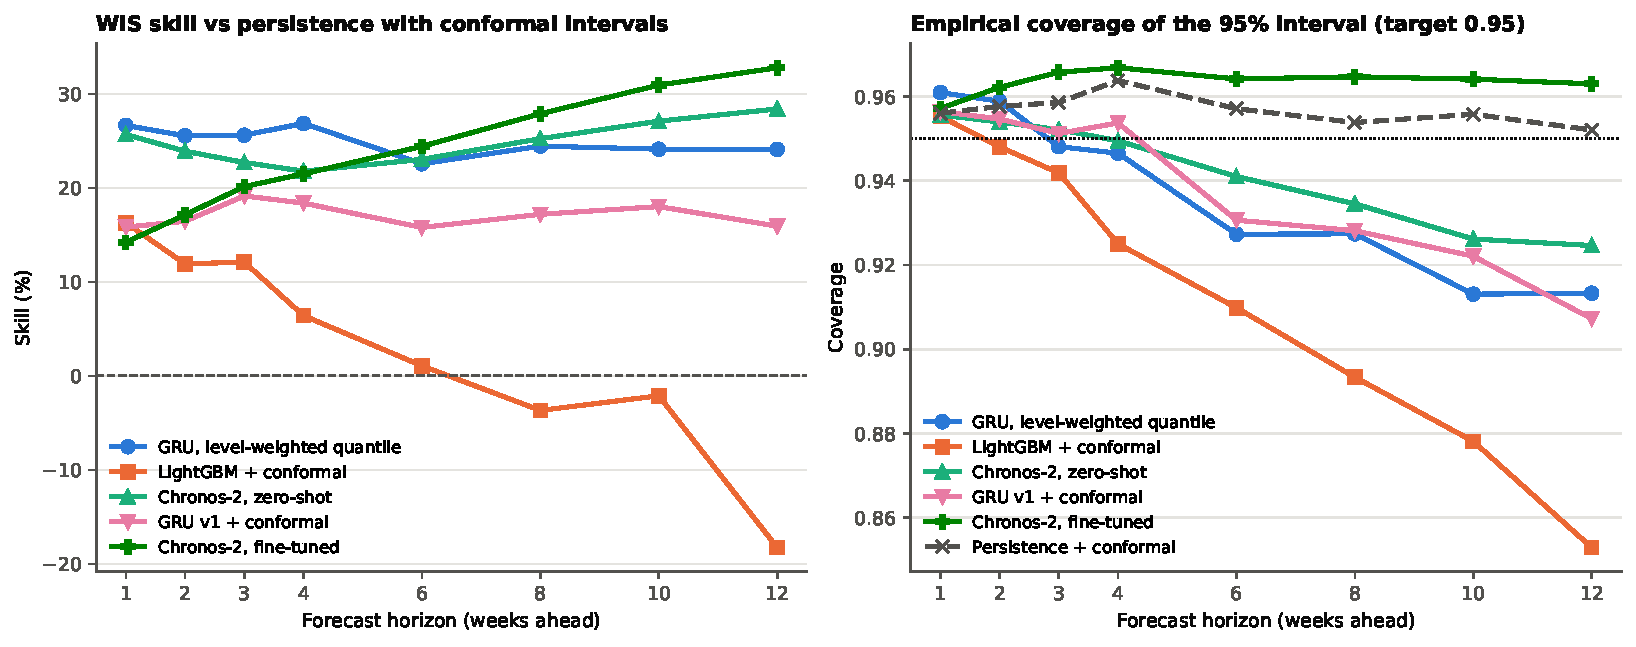
\includegraphics[width=\textwidth]{fig_lh_probabilistic}
\caption{WIS skill relative to persistence with conformal intervals (left) and empirical coverage of the 95\% interval (right, target dotted).}
\label{fig:probabilistic}
\Description{Left: weighted interval score skill versus horizon, native quantile forecasts highest. Right: 95 percent interval coverage versus horizon, with conformal intervals of trained point models falling below 0.95 at long horizons.}
\end{figure*}

Native quantile forecasts are the best probabilistic forecasts at every horizon (Table~\ref{tab:wis}, Figure~\ref{fig:probabilistic}), improving WIS over persistence by 27\% at one and four weeks and by 33\% at twelve. Chronos-2's intervals are calibrated as produced, at 0.93--0.96 coverage across horizons; recalibrating them on the previous year makes WIS slightly worse. Conformal intervals built from the previous year's errors under-cover at long horizons for the trained point models (0.85--0.89 at 10--12 weeks), because error distributions shift between epidemic and quiet years. Persistence's intervals do not suffer this, which suggests the trained models' errors are less stationary than their accuracy gains alone would indicate.

%% ---------------------------------------------------------------------------
\section{Early Warning: Outbreak Weeks versus Onsets}
\label{sec:ews}

\begin{table}[t]
\centering
\caption{ROC-AUC for outbreak weeks (vs all other weeks) and for outbreak onsets (vs quiet weeks).}
\label{tab:ews}
\begin{tabular}{lcccccc}
\toprule
& \multicolumn{3}{c}{\textbf{Outbreak week}} & \multicolumn{3}{c}{\textbf{Onset}} \\
\textbf{Method} & $h$=1 & 4 & 12 & 1 & 4 & 12 \\
\midrule
Persistence & 0.89 & 0.81 & 0.60 & 0.60 & 0.52 & 0.44 \\
Climatology & 0.65 & 0.65 & 0.65 & 0.61 & 0.61 & 0.61 \\
GRU v2 & 0.91 & 0.86 & 0.70 & 0.61 & 0.61 & 0.56 \\
Chronos-2 joint, FT & 0.91 & 0.85 & 0.71 & 0.63 & 0.60 & 0.56 \\
\bottomrule
\end{tabular}
\end{table}

\begin{figure*}[t]
\centering
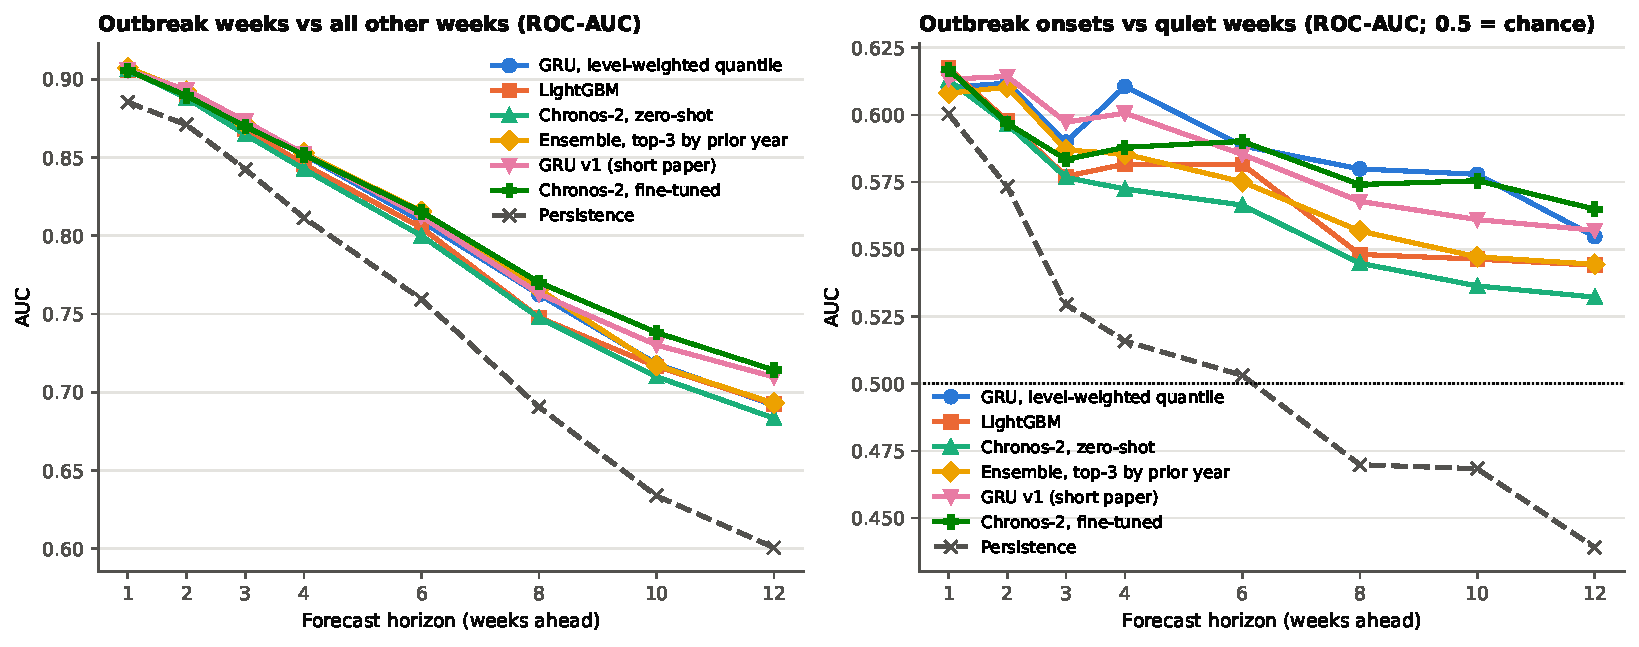
\includegraphics[width=\textwidth]{fig_lh_early_warning}
\caption{Discrimination of outbreak weeks (left) and of outbreak onsets against quiet weeks (right); 0.5 is chance.}
\label{fig:ews}
\Description{Left: outbreak-week ROC-AUC falling from about 0.9 at one week to 0.6 to 0.7 at twelve weeks. Right: onset ROC-AUC between about 0.45 and 0.63 for all methods, close to the 0.5 chance line.}
\end{figure*}

Learned models discriminate outbreak weeks well, at AUC 0.91 one week ahead against 0.89 for persistence, and the gap widens with horizon (0.70--0.71 against 0.60 at twelve weeks). Predicting \emph{onsets} is a different matter (Table~\ref{tab:ews}, Figure~\ref{fig:ews}). Onset AUC is 0.60--0.63 at one week and 0.53--0.57 at twelve for every method, persistence falls below chance at long horizons, and a five-year seasonal average predicts onsets about as well as any model. High outbreak-detection scores therefore mostly reflect outbreaks already under way.

The practical rule ``warn when the forecast crosses the threshold'' detects 0--7\% of onsets, because point forecasts are conditional medians that lag turning points. With each method's alarm cutoff set on the previous year to give a 10\% false-alarm rate, models detect about 20--25\% of onsets against 10--24\% for persistence, and realised false-alarm rates run near 20\%, again reflecting year-to-year non-stationarity.

\textbf{A dedicated onset classifier.} We trained a LightGBM classifier only on origins where the district is currently below its threshold, predicting whether it will be above threshold $h$ weeks later. On those rows it has the best onset AUC at one week (0.70 against 0.67--0.69 for the forecasters) but not at four (0.66 against 0.69 for the GRU). Climate helps it (0.66 against 0.62 without climate at four weeks; 0.65 against 0.61 at six), consistent with weather driving transitions. The ceiling remains about 0.65--0.70.

%% ---------------------------------------------------------------------------
\section{Discussion}

\textbf{Where the skill is.} Persistence is a strong baseline at one week because dengue incidence is highly autocorrelated. Beyond two weeks the latest count goes stale faster than learned forecasts degrade, and climate, seasonal phase and cross-district context supply real information. Published comparisons that omit persistence cannot distinguish these regimes.

\textbf{Foundation models as baselines.} A zero-shot foundation model that has never seen dengue matches a purpose-built model trained on nineteen years of Sri Lankan data, and gives calibrated intervals for free. New dengue forecasting models should report a foundation-model baseline alongside persistence. Fine-tuning on pre-epidemic years illustrates a risk: domain adaptation can lower robustness to regime change.

\textbf{Graphs.} Across contiguity, distance and learned adjacencies, and across all horizons, graph convolution did not help. This contrasts with reported GNN gains for Sri Lanka~\cite{weng2024graph,gulmohamed2026denguegnn}, which were measured against weaker baselines and without a no-graph control.

\textbf{Operational use.} For planning horizons of one to three months, the ensemble or Chronos-2 forecasts with native intervals are the most useful outputs. For early warning of new outbreaks, current case and weather data support modest discrimination at best; mobility, entomological or serotype data are likely needed.

\textbf{Limitations.} The benchmark climate is a centroid-based reconstruction of ERA5 rather than the original polygon means. Seven headline years give low statistical power, and many arms were compared, so the one-week result needs replication. Chronos fine-tuning was tuned on a single validation year. The outbreak threshold is a statistical percentile rather than an official epidemic threshold.

%% ---------------------------------------------------------------------------
\section{Conclusion}

A leakage-controlled benchmark of 24 forecasters for 25 Sri Lankan districts shows that forecasting skill over persistence is small at one week and substantial from three to twelve weeks, reaching 19--25\% MAE skill and 27--33\% WIS improvement. Climate contributes from two to four weeks ahead onward in three model families, spatial graphs never help, and a zero-shot foundation model rivals a purpose-built GRU. The same models that recognise ongoing outbreaks remain close to chance at predicting when outbreaks start. Future work should target onset prediction with additional data sources, test the one-week result on held-out years, and evaluate the forecasts prospectively with the NDCU.

\bibliographystyle{ACM-Reference-Format}
\bibliography{references_long}

\end{document}
